\newpage
\subsection{例題4-1 ミニサッカーゲームの人を\ruby{改造}{かい|ぞう}する}

\begin{description}
    \item \textgt{\bf 考え方}
\end{description}

ミニサッカーゲーム(kick.hsp)のプログラムを改造してゲームの内容を変えてみましょう。

このゲームに\ruby{登場}{とう|じょう}する人は、実は文字の組み合わせで作られています。

\ruby{顔文字}{かお|も|じ}(\^{}\^{}) みたいですね。


\begin{figure}[H]
    \begin{center}
      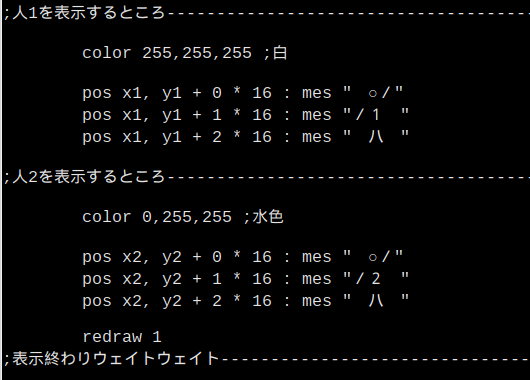
\includegraphics[keepaspectratio,width=12.326cm,height=8.123cm]{text04-img/text04-img007.png}
      \caption{ミニサッカーゲームのプログラム}
    \end{center}
    \label{fig:prog_menu}
\end{figure}



プログラムから、mes命令で人を表示している部分を探して改造してみましょう。

mes命令は、

\begin{description}
    \item \textgt{\bf mes \ “文字”}
\end{description}


のように必ず「”」の記号で文字を囲む必要があるので忘れないでください。

\begin{description}
    \item \textgt{\bf 例題1 答え}
\end{description}


[F5]キーを押して改造した人がきちんと表示されるかどうか確認しましょう。

\ \ \ \ 人を改造することで、見た目が変わってあなただけのゲームに変わります。

改造ができたらTAや周りの友達にも見せてあげましょう。

\clearpage





